% Costo de las ranuras. GENERADO por recursos_ranuras.py desde
% recursos_ranuras.csv: no editar a mano.
\documentclass[border=0pt,tikz]{standalone}
\usepackage[utf8]{inputenc}
\usepackage[T1]{fontenc}
\usepackage{lmodern}
\usepackage[none]{hyphenat}
% Estilo común de las figuras TikZ (panoramas y diagramas de bloques).
%
% Cada figura lo incluye con \input{../../figuras/estilo_tikz.tex} (las figuras
% viven en docs/<módulo>/figuras/). Un solo lugar para la paleta, los estilos de
% bloque y el formato de los parámetros: si cambia algo acá, cambia en todas.
%
% La paleta es la misma de docs/figuras/estilo_svg.py y de PALETA en
% modulos/mk/datasheet.py; si se toca un color, se toca en los tres.
%
% Requiere: \usepackage{tikz} (lo da la clase standalone con la opción tikz).

\usetikzlibrary{arrows.meta,positioning,calc,fit,backgrounds,shapes.multipart,
                decorations.markings,shadows}

% ---------------------------------------------------------------- colores ---
\definecolor{azul}{RGB}{108,172,228}      % acondicionamiento
\definecolor{verde}{RGB}{110,214,142}     % captura / histogramas en BRAM
\definecolor{amarillo}{RGB}{252,232,160}  % trigger
\definecolor{naranja}{RGB}{252,206,160}   % camino a DDR
\definecolor{grisr}{RGB}{226,226,226}     % compartido / infraestructura
\definecolor{rojo}{RGB}{240,128,128}      % bus del sistema

% ---------------------------------------------------------------- estilos ---
\tikzset{
  >={Stealth[length=2.4mm,width=1.8mm]},
  % fondo blanco siempre: el SVG se ve igual en modo claro y oscuro
  fondo/.style   = {show background rectangle, inner frame sep=8pt,
                    background rectangle/.style={fill=white, draw=none}},
  bloque/.style  = {draw=black, line width=0.6pt, rounded corners=2pt,
                    align=center, text width=2.2cm, minimum height=1.15cm,
                    inner sep=2pt, font=\scriptsize, fill=#1},
  datos/.style   = {bloque=azul!35},
  trig/.style    = {bloque=amarillo},
  captura/.style = {bloque=verde!55},
  ddr/.style     = {bloque=naranja!70},
  comp/.style    = {bloque=grisr},
  bus/.style     = {bloque=rojo!45},
  % lógica escrita dentro del módulo, sin submódulo propio
  etapa/.style   = {bloque=#1, line width=0.5pt},
  etapa/.default = verde!20,
  % lo que el bitstream no trae (atado a cero, stub, salida muda)
  mudo/.style    = {bloque=white, draw=black!45, dashed, text=black!55},
  %
  % BLOQUE CON PARÁMETROS, en el formato del datasheet: el encabezado lleva el
  % nombre y los parámetros con que lo instancia el padre (NOMBRE=valor, en
  % monoespaciada, uno por línea); el cuerpo, más claro, lo que hace.
  %   \node[datos, param={azul!35}{azul!12}] {\blk{nombre}{} \prm{A=1\\B=2}
  %                                            \nodepart{two} función};
  param/.style 2 args = {rectangle split, rectangle split parts=2,
                         rectangle split part fill={#1, #2}},
  %
  flujo/.style   = {->, line width=0.8pt},
  ctrl/.style    = {->, line width=0.6pt, black!65},
  % la línea que pasa por encima en un cruce: un halo blanco la separa
  cruce/.style   = {preaction={draw=white, line width=3.4pt, -}},
  % marca de ancho de bus: barra oblicua a mitad de la flecha, con el número
  % encima. \draw[flujo, ancho=14] ...; para otra posición, ancho en=0.3.
  ancho/.style   = {decoration={markings, mark=at position \anchopos with {
                      \draw[line width=0.6pt, -] (-0.1,-0.14) -- (0.1,0.14);
                      \node[font=\scriptsize, above=1.5pt] {#1};}},
                    postaction={decorate}},
  % la misma marca en una flecha vertical: el número va a la derecha
  anchov/.style  = {decoration={markings, mark=at position \anchopos with {
                      \draw[line width=0.6pt, -] (-0.14,-0.1) -- (0.14,0.1);
                      \node[font=\scriptsize, right=3pt] {#1};}},
                    postaction={decorate}},
  ancho en/.code = {\def\anchopos{#1}},
  sen/.style     = {font=\scriptsize\ttfamily, inner sep=1.5pt},
  nodo/.style    = {font=\tiny\ttfamily, inner sep=1pt, black!75},
  pin/.style     = {font=\scriptsize, align=center, inner sep=1pt},
  grupo/.style   = {draw=black!55, dashed, line width=0.7pt, rounded corners=4pt},
  canal/.style   = {grupo},
  contenedor/.style = {draw=black!80, line width=1.0pt, rounded corners=6pt},
  % marca numerada: cada número es una fila de la tabla del documento
  marca/.style   = {circle, fill=black, text=white, font=\scriptsize\bfseries,
                    inner sep=0pt, minimum size=4.3mm},
  %
  % DECISIONES (docs/mca/vista_general_mca.md). Cada opción es un bloque, todas
  % entran a un mux (\muxdec, abajo) y el registro que elige entra por abajo.
  % la opción que trae el reset (el comportamiento histórico): borde doble
  defecto/.style = {double=white, double distance=0.8pt, line width=0.45pt},
  % rótulo de la decisión, el mismo Dn del panorama y del documento
  decision/.style = {circle, fill=black, text=white, font=\small\bfseries,
                     inner sep=0pt, minimum size=7mm},
  %
  % LÓGICA (docs/mca/figuras/contabilidad/ y los detalles de las decisiones)
  % registro: caja gris con el triángulo de reloj en el borde de abajo
  registro/.style = {draw=black, line width=0.6pt, fill=grisr, align=center,
                     font=\scriptsize, inner sep=2pt, minimum width=#1,
                     minimum height=0.85cm,
                     path picture={\draw[line width=0.5pt]
                       ([xshift=-1.1mm]path picture bounding box.south) --
                       ([yshift=1.6mm]path picture bounding box.south) --
                       ([xshift=1.1mm]path picture bounding box.south);}},
  registro/.default = 0.8cm,
  % condición de una cadena if / else-if: "sí" sale a la derecha, "no" abajo
  pregunta/.style = {draw=black, line width=0.5pt, rounded corners=7pt,
                     fill=white, font=\scriptsize\ttfamily, align=center,
                     inner sep=2.5pt, minimum height=0.62cm, text width=#1},
  pregunta/.default = 1.9cm,
  si/.style      = {font=\tiny, inner sep=1pt, above, pos=0.12},
  no/.style      = {font=\tiny, inner sep=1pt, left, pos=0.45},
  %
  titulo/.style  = {anchor=north west, font=\small, inner sep=4pt, align=left},
  rotulo/.style  = {anchor=north west, font=\scriptsize\itshape, black!70,
                    inner sep=2pt, align=left},
}

% submódulo: nombre en monoespaciada; lógica propia: nombre en romana
\newcommand{\blk}[2]{{\ttfamily\bfseries #1}\\[1pt]#2}
\newcommand{\etq}[2]{{\bfseries #1}\\[1pt]#2}
\newcommand{\punto}[1]{\fill (#1) circle (1.3pt);}

% Parámetros en el formato del datasheet: NOMBRE=valor en monoespaciada, una
% entrada por celda, hasta cuatro columnas. Una columna: \prm{A=1\\B=2};
% dos: \prm{A=1 & B=2\\C=3}.
\newcommand{\prm}[1]{{\ttfamily\fontsize{5.6}{6.6}\selectfont
  \begin{tabular}{@{}l@{\hspace{7pt}}l@{\hspace{7pt}}l@{\hspace{7pt}}l@{}}#1\end{tabular}}}

\def\anchopos{0.5}

% Mux de una decisión: trapecio con el lado ancho (las entradas) a la izquierda.
% #1 = nombre, #2 = centro, #3 = alto en cm. Deja tres coordenadas:
%   (#1-in)  centro del lado de entradas: las flechas llegan a (#1-in |- opcion.east)
%   (#1-out) la salida
%   (#1-sel) mitad del lado de abajo: por ahí entra el registro que elige
% El rótulo de adentro es opcional: \muxdec{m}{(4,0)}{3.6} y después
% \node[...] at (m) {...}.
\newcommand{\muxdec}[3]{%
  \path #2 coordinate (#1);
  \draw[line width=0.6pt, fill=grisr]
    ($(#1)+(-0.45,{#3/2})$) -- ($(#1)+(0.45,{#3/2-0.35})$) --
    ($(#1)+(0.45,{-#3/2+0.35})$) -- ($(#1)+(-0.45,{-#3/2})$) -- cycle;
  \coordinate (#1-in)  at ($(#1)+(-0.45,0)$);
  \coordinate (#1-out) at ($(#1)+(0.45,0)$);
  \coordinate (#1-sel) at ($(#1)+(0,{-#3/2+0.175})$);}

% El mismo mux rotado 90 grados, para un flujo de arriba hacia abajo: entradas
% por el lado ancho de arriba, salida abajo y el registro que elige por la
% izquierda. #1 = nombre, #2 = centro, #3 = ancho en cm. Deja (#1-in) centro del
% lado de entradas, (#1-out) la salida y (#1-sel) mitad del lado izquierdo.
\newcommand{\muxdecv}[3]{%
  \path #2 coordinate (#1);
  \draw[line width=0.6pt, fill=grisr]
    ($(#1)+({-#3/2},0.45)$) -- ($(#1)+({#3/2},0.45)$) --
    ($(#1)+({#3/2-0.35},-0.45)$) -- ($(#1)+({-#3/2+0.35},-0.45)$) -- cycle;
  \coordinate (#1-in)  at ($(#1)+(0,0.45)$);
  \coordinate (#1-out) at ($(#1)+(0,-0.45)$);
  \coordinate (#1-sel) at ($(#1)+({-#3/2+0.175},0)$);}

% Leyenda de colores + nota. #1 = posición, #2 = color/texto, #3 = nota.
\newcommand{\leyenda}[3]{%
  \begin{scope}[shift={(#1)}, every node/.style={font=\scriptsize}]
    \coordinate (t0) at (-0.5,0);
    \foreach \c/\t [count=\i] in {#2} {
      \pgfmathtruncatemacro\j{\i-1}
      \node[draw, fill=\c, minimum width=4mm, minimum height=3mm, inner sep=0pt,
            right=5mm of t\j.east, anchor=west] (l\i) {};
      \node[right=1.5mm of l\i] (t\i) {\t};
    }
    \node[anchor=north west, black!70, text width=19cm, align=left]
      at (-0.05,-0.3) {#3};
  \end{scope}}

% Lo que dicen los parámetros, para la nota de la leyenda
\newcommand{\notaparam}{\texttt{NOMBRE=valor}: parámetros con que el padre
  instancia el bloque (se omiten los que sólo pasan el del padre sin cambio).}

\begin{document}
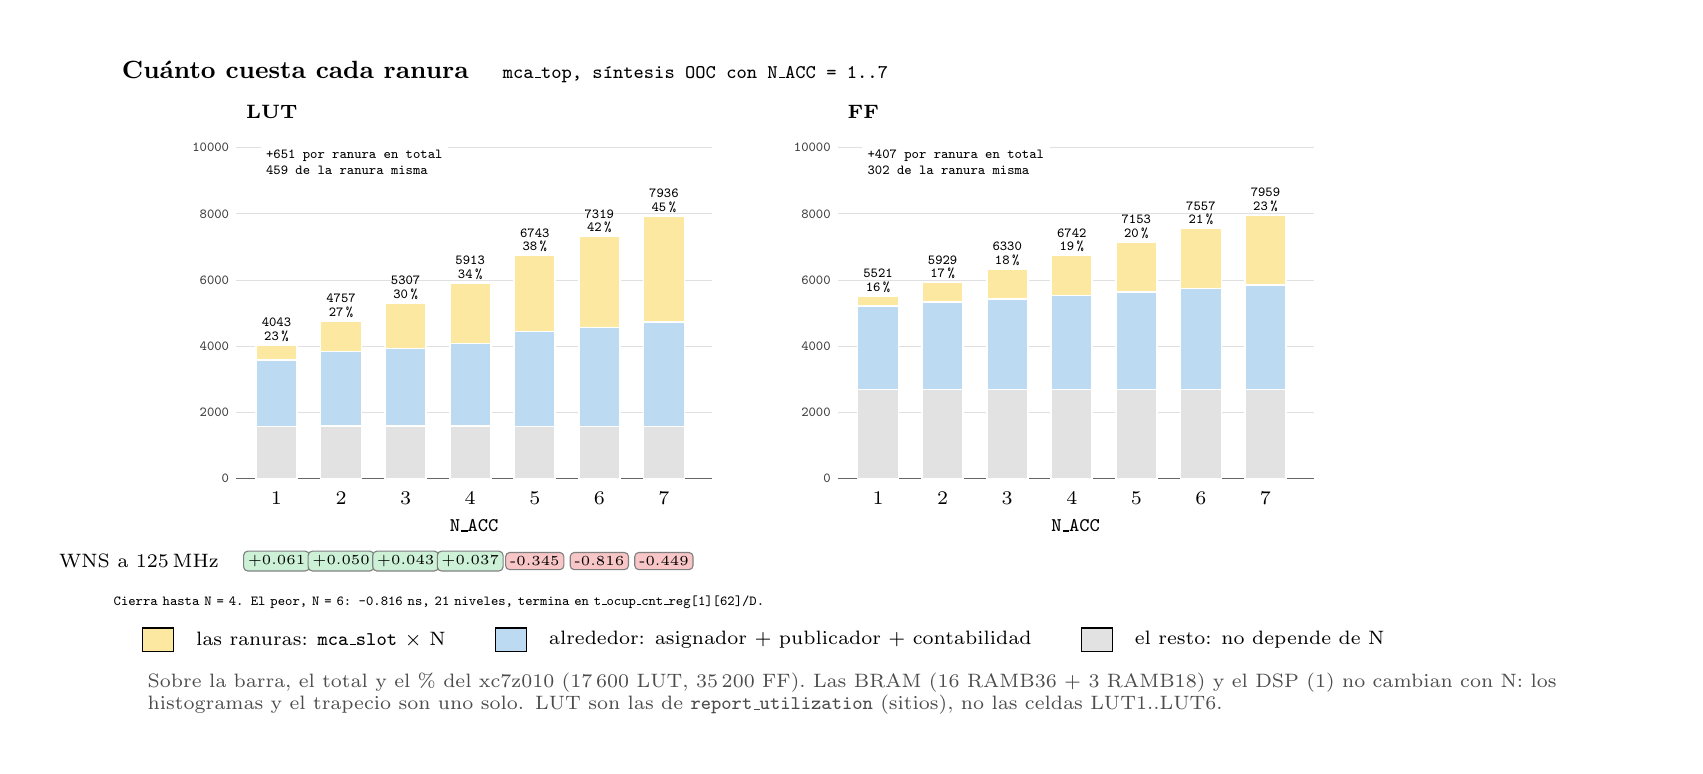
\begin{tikzpicture}[fondo]
\node[titulo] at (-1.6,5.45) {\textbf{Cuánto cuesta cada ranura} \quad {\scriptsize\ttfamily mca\_top, síntesis OOC con N\_ACC = 1..7}};
\node[anchor=south west, font=\scriptsize\bfseries] at (0.00,4.45) {LUT};
\draw[black!12, line width=0.3pt] (0.00,0.000) -- (6.04,0.000);
\node[nodo, anchor=east] at (-0.05,0.000) {0};
\draw[black!12, line width=0.3pt] (0.00,0.840) -- (6.04,0.840);
\node[nodo, anchor=east] at (-0.05,0.840) {2000};
\draw[black!12, line width=0.3pt] (0.00,1.680) -- (6.04,1.680);
\node[nodo, anchor=east] at (-0.05,1.680) {4000};
\draw[black!12, line width=0.3pt] (0.00,2.520) -- (6.04,2.520);
\node[nodo, anchor=east] at (-0.05,2.520) {6000};
\draw[black!12, line width=0.3pt] (0.00,3.360) -- (6.04,3.360);
\node[nodo, anchor=east] at (-0.05,3.360) {8000};
\draw[black!12, line width=0.3pt] (0.00,4.200) -- (6.04,4.200);
\node[nodo, anchor=east] at (-0.05,4.200) {10000};
\draw[black!60, line width=0.5pt] (0.00,0) -- (6.04,0);
\draw[fill=grisr, draw=white, line width=0.6pt] (0.250,0.000) rectangle (0.770,0.661);
\draw[fill=azul!45, draw=white, line width=0.6pt] (0.250,0.661) rectangle (0.770,1.504);
\draw[fill=amarillo, draw=white, line width=0.6pt] (0.250,1.504) rectangle (0.770,1.698);
\node[nodo, black, anchor=south, align=center] at (0.510,1.698) {4043\\[-1pt]23\,\%};
\node[font=\scriptsize, anchor=north] at (0.510,-0.05) {1};
\draw[fill=grisr, draw=white, line width=0.6pt] (1.070,0.000) rectangle (1.590,0.662);
\draw[fill=azul!45, draw=white, line width=0.6pt] (1.070,0.662) rectangle (1.590,1.612);
\draw[fill=amarillo, draw=white, line width=0.6pt] (1.070,1.612) rectangle (1.590,1.998);
\node[nodo, black, anchor=south, align=center] at (1.330,1.998) {4757\\[-1pt]27\,\%};
\node[font=\scriptsize, anchor=north] at (1.330,-0.05) {2};
\draw[fill=grisr, draw=white, line width=0.6pt] (1.890,0.000) rectangle (2.410,0.662);
\draw[fill=azul!45, draw=white, line width=0.6pt] (1.890,0.662) rectangle (2.410,1.651);
\draw[fill=amarillo, draw=white, line width=0.6pt] (1.890,1.651) rectangle (2.410,2.229);
\node[nodo, black, anchor=south, align=center] at (2.150,2.229) {5307\\[-1pt]30\,\%};
\node[font=\scriptsize, anchor=north] at (2.150,-0.05) {3};
\draw[fill=grisr, draw=white, line width=0.6pt] (2.710,0.000) rectangle (3.230,0.662);
\draw[fill=azul!45, draw=white, line width=0.6pt] (2.710,0.662) rectangle (3.230,1.711);
\draw[fill=amarillo, draw=white, line width=0.6pt] (2.710,1.711) rectangle (3.230,2.483);
\node[nodo, black, anchor=south, align=center] at (2.970,2.483) {5913\\[-1pt]34\,\%};
\node[font=\scriptsize, anchor=north] at (2.970,-0.05) {4};
\draw[fill=grisr, draw=white, line width=0.6pt] (3.530,0.000) rectangle (4.050,0.661);
\draw[fill=azul!45, draw=white, line width=0.6pt] (3.530,0.661) rectangle (4.050,1.866);
\draw[fill=amarillo, draw=white, line width=0.6pt] (3.530,1.866) rectangle (4.050,2.832);
\node[nodo, black, anchor=south, align=center] at (3.790,2.832) {6743\\[-1pt]38\,\%};
\node[font=\scriptsize, anchor=north] at (3.790,-0.05) {5};
\draw[fill=grisr, draw=white, line width=0.6pt] (4.350,0.000) rectangle (4.870,0.661);
\draw[fill=azul!45, draw=white, line width=0.6pt] (4.350,0.661) rectangle (4.870,1.915);
\draw[fill=amarillo, draw=white, line width=0.6pt] (4.350,1.915) rectangle (4.870,3.074);
\node[nodo, black, anchor=south, align=center] at (4.610,3.074) {7319\\[-1pt]42\,\%};
\node[font=\scriptsize, anchor=north] at (4.610,-0.05) {6};
\draw[fill=grisr, draw=white, line width=0.6pt] (5.170,0.000) rectangle (5.690,0.661);
\draw[fill=azul!45, draw=white, line width=0.6pt] (5.170,0.661) rectangle (5.690,1.985);
\draw[fill=amarillo, draw=white, line width=0.6pt] (5.170,1.985) rectangle (5.690,3.333);
\node[nodo, black, anchor=south, align=center] at (5.430,3.333) {7936\\[-1pt]45\,\%};
\node[font=\scriptsize, anchor=north] at (5.430,-0.05) {7};
\node[font=\scriptsize, anchor=north] at (3.02,-0.4) {\texttt{N\_ACC}};
\node[nodo, black, anchor=north west, align=left, fill=white, inner sep=2pt] at (0.30,4.25) {+651 por ranura en total\\459 de la ranura misma};
\node[anchor=south west, font=\scriptsize\bfseries] at (7.64,4.45) {FF};
\draw[black!12, line width=0.3pt] (7.64,0.000) -- (13.68,0.000);
\node[nodo, anchor=east] at (7.59,0.000) {0};
\draw[black!12, line width=0.3pt] (7.64,0.840) -- (13.68,0.840);
\node[nodo, anchor=east] at (7.59,0.840) {2000};
\draw[black!12, line width=0.3pt] (7.64,1.680) -- (13.68,1.680);
\node[nodo, anchor=east] at (7.59,1.680) {4000};
\draw[black!12, line width=0.3pt] (7.64,2.520) -- (13.68,2.520);
\node[nodo, anchor=east] at (7.59,2.520) {6000};
\draw[black!12, line width=0.3pt] (7.64,3.360) -- (13.68,3.360);
\node[nodo, anchor=east] at (7.59,3.360) {8000};
\draw[black!12, line width=0.3pt] (7.64,4.200) -- (13.68,4.200);
\node[nodo, anchor=east] at (7.59,4.200) {10000};
\draw[black!60, line width=0.5pt] (7.64,0) -- (13.68,0);
\draw[fill=grisr, draw=white, line width=0.6pt] (7.890,0.000) rectangle (8.410,1.128);
\draw[fill=azul!45, draw=white, line width=0.6pt] (7.890,1.128) rectangle (8.410,2.193);
\draw[fill=amarillo, draw=white, line width=0.6pt] (7.890,2.193) rectangle (8.410,2.319);
\node[nodo, black, anchor=south, align=center] at (8.150,2.319) {5521\\[-1pt]16\,\%};
\node[font=\scriptsize, anchor=north] at (8.150,-0.05) {1};
\draw[fill=grisr, draw=white, line width=0.6pt] (8.710,0.000) rectangle (9.230,1.128);
\draw[fill=azul!45, draw=white, line width=0.6pt] (8.710,1.128) rectangle (9.230,2.237);
\draw[fill=amarillo, draw=white, line width=0.6pt] (8.710,2.237) rectangle (9.230,2.490);
\node[nodo, black, anchor=south, align=center] at (8.970,2.490) {5929\\[-1pt]17\,\%};
\node[font=\scriptsize, anchor=north] at (8.970,-0.05) {2};
\draw[fill=grisr, draw=white, line width=0.6pt] (9.530,0.000) rectangle (10.050,1.128);
\draw[fill=azul!45, draw=white, line width=0.6pt] (9.530,1.128) rectangle (10.050,2.279);
\draw[fill=amarillo, draw=white, line width=0.6pt] (9.530,2.279) rectangle (10.050,2.659);
\node[nodo, black, anchor=south, align=center] at (9.790,2.659) {6330\\[-1pt]18\,\%};
\node[font=\scriptsize, anchor=north] at (9.790,-0.05) {3};
\draw[fill=grisr, draw=white, line width=0.6pt] (10.350,0.000) rectangle (10.870,1.128);
\draw[fill=azul!45, draw=white, line width=0.6pt] (10.350,1.128) rectangle (10.870,2.324);
\draw[fill=amarillo, draw=white, line width=0.6pt] (10.350,2.324) rectangle (10.870,2.832);
\node[nodo, black, anchor=south, align=center] at (10.610,2.832) {6742\\[-1pt]19\,\%};
\node[font=\scriptsize, anchor=north] at (10.610,-0.05) {4};
\draw[fill=grisr, draw=white, line width=0.6pt] (11.170,0.000) rectangle (11.690,1.128);
\draw[fill=azul!45, draw=white, line width=0.6pt] (11.170,1.128) rectangle (11.690,2.370);
\draw[fill=amarillo, draw=white, line width=0.6pt] (11.170,2.370) rectangle (11.690,3.004);
\node[nodo, black, anchor=south, align=center] at (11.430,3.004) {7153\\[-1pt]20\,\%};
\node[font=\scriptsize, anchor=north] at (11.430,-0.05) {5};
\draw[fill=grisr, draw=white, line width=0.6pt] (11.990,0.000) rectangle (12.510,1.128);
\draw[fill=azul!45, draw=white, line width=0.6pt] (11.990,1.128) rectangle (12.510,2.413);
\draw[fill=amarillo, draw=white, line width=0.6pt] (11.990,2.413) rectangle (12.510,3.174);
\node[nodo, black, anchor=south, align=center] at (12.250,3.174) {7557\\[-1pt]21\,\%};
\node[font=\scriptsize, anchor=north] at (12.250,-0.05) {6};
\draw[fill=grisr, draw=white, line width=0.6pt] (12.810,0.000) rectangle (13.330,1.128);
\draw[fill=azul!45, draw=white, line width=0.6pt] (12.810,1.128) rectangle (13.330,2.455);
\draw[fill=amarillo, draw=white, line width=0.6pt] (12.810,2.455) rectangle (13.330,3.343);
\node[nodo, black, anchor=south, align=center] at (13.070,3.343) {7959\\[-1pt]23\,\%};
\node[font=\scriptsize, anchor=north] at (13.070,-0.05) {7};
\node[font=\scriptsize, anchor=north] at (10.66,-0.4) {\texttt{N\_ACC}};
\node[nodo, black, anchor=north west, align=left, fill=white, inner sep=2pt] at (7.94,4.25) {+407 por ranura en total\\302 de la ranura misma};
\node[anchor=east, font=\scriptsize] at (-0.10,-1.05) {WNS a 125\,MHz};
\node[draw=black!50, fill=verde!35, rounded corners=1.5pt, font=\tiny, minimum width=0.74cm, inner sep=1.5pt] at (0.510,-1.05) {+0.061};
\node[draw=black!50, fill=verde!35, rounded corners=1.5pt, font=\tiny, minimum width=0.74cm, inner sep=1.5pt] at (1.330,-1.05) {+0.050};
\node[draw=black!50, fill=verde!35, rounded corners=1.5pt, font=\tiny, minimum width=0.74cm, inner sep=1.5pt] at (2.150,-1.05) {+0.043};
\node[draw=black!50, fill=verde!35, rounded corners=1.5pt, font=\tiny, minimum width=0.74cm, inner sep=1.5pt] at (2.970,-1.05) {+0.037};
\node[draw=black!50, fill=rojo!45, rounded corners=1.5pt, font=\tiny, minimum width=0.74cm, inner sep=1.5pt] at (3.790,-1.05) {-0.345};
\node[draw=black!50, fill=rojo!45, rounded corners=1.5pt, font=\tiny, minimum width=0.74cm, inner sep=1.5pt] at (4.610,-1.05) {-0.816};
\node[draw=black!50, fill=rojo!45, rounded corners=1.5pt, font=\tiny, minimum width=0.74cm, inner sep=1.5pt] at (5.430,-1.05) {-0.449};
\node[nodo, black, anchor=north west, text width=14.7cm] at (-1.6,-1.45) {Cierra hasta N = 4. El peor, N = 6: -0.816 ns, 21 niveles, termina en \texttt{t\_ocup\_cnt\_reg[1][62]/D}.};
\leyenda{-1.2,-2.05}{amarillo/las ranuras: \texttt{mca\_slot} $\times$ N, azul!45/alrededor: asignador + publicador + contabilidad, grisr/el resto: no depende de N}
  {Sobre la barra, el total y el \% del xc7z010 (17\,600 LUT, 35\,200 FF). Las BRAM (16 RAMB36 + 3 RAMB18) y el DSP (1) no cambian con N: los histogramas y el trapecio son uno solo. LUT son las de \texttt{report\_utilization} (sitios), no las celdas LUT1..LUT6.}
\end{tikzpicture}
\end{document}
